%initialising document, adjust papersize, fontsize and page orientation to your needs
\documentclass[a4paper, fontsize = 8pt, landscape]{scrartcl}
\usepackage{../../../misc_files/LateX/layout_and_colours}
\title{Algorithmen und Datenstrukturen}
\author{Jil Zerndt, Lucien Perret}
\date{May 2024}

\createtitlepagestyle
\createmainpagestyle
\begin{document}
\begin{multicols}{3}
	\thispagestyle{TitlePageStyle}
	\maketitle
	%


\section{Overview of IT Security}

\mult{2}

\begin{definition}{Key IT Security Goals}
Information security is based on three fundamental principles, commonly known as the CIA triad:
\begin{itemize}
    \item \textbf{Confidentiality} - Ensuring data is only accessible to authorized users
    \item \textbf{Integrity} - Ensuring data is not modified in an unauthorized way
    \item \textbf{Availability} - Ensuring systems and data are accessible when needed
\end{itemize}
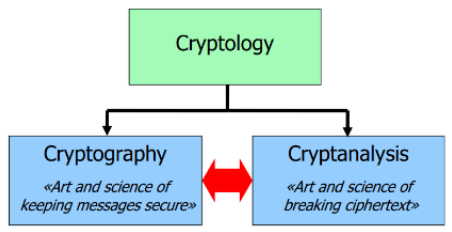
\includegraphics[width=0.6\linewidth]{its_goals.png}
\end{definition}

\begin{concept}{Business IT Risks}
\begin{itemize}
    \item Data loss
    \item System outage
    \item Espionage
    \item Sabotage
    \item Reputation loss
    \item Misuse of computing resources
    \item Violation of regulations
    \item Fraud
    \item Brand misuse
    \item Ransom demands
\end{itemize}
These risks can have significant financial, operational, and reputational impacts.
\end{concept}

\multend

\raggedcolumns

\subsubsection{Security Frameworks and Controls}

\mult{2}

\begin{concept}{Security Control Frameworks}
Security frameworks provide structured approaches to implementing security controls:
\begin{itemize}
    \item \textbf{CIS Controls} - Prioritized set of actions to protect organizations
    \item Controls are typically organized in implementation groups based on difficulty and impact
    \item Focus on preventing the most common attack vectors first
\end{itemize}
\end{concept}

\begin{definition}{Types of Security Measures}
Security measures can be categorized based on their focus:
\begin{itemize}
    \item \textbf{Preventive} - Block threats before they occur (firewalls, access controls)
    \item \textbf{Detective} - Identify when a breach has occurred (IDS, audit logs)
    \item \textbf{Corrective} - Mitigate damage after an incident (backups, incident response)
\end{itemize}
\end{definition}

\multend

\subsubsection{Disaster Recovery}



\begin{concept}{Business Continuity Management}
Disaster recovery and business continuity planning are essential for maintaining availability:
\begin{itemize}
    \item \textbf{Recovery Plan} - Detailed procedures for recovering from incidents
    \item \textbf{Recovery Tests} - Regular testing of recovery procedures
    \item \textbf{Redundancy} - Duplicate systems, power supplies, and network connections
    \item \textbf{Offline backups} - Protection against ransomware and other threats
\end{itemize}
\end{concept}

\begin{KR}{Disaster Recovery Planning}
\paragraph{Initial Assessment}
\begin{itemize}
    \item Identify critical systems and data
    \item Determine acceptable recovery time objectives (RTO)
    \item Determine acceptable recovery point objectives (RPO)
\end{itemize}

\paragraph{Plan Development}
\begin{itemize}
    \item Document recovery procedures
    \item Assign roles and responsibilities
    \item Include contact details for all relevant parties
    \item Develop technical instructions for restoration
\end{itemize}

\paragraph{Testing}
\begin{itemize}
    \item Conduct regular theoretical dry runs
    \item Perform practical tests (e.g., server shutdown, data restoration)
    \item Update procedures based on test results
\end{itemize}

\paragraph{Regular Review}
\begin{itemize}
    \item Review and update plans regularly
    \item Consider changes in infrastructure, personnel, and threats
\end{itemize}
\end{KR}

\begin{example}
A medium-sized company implements a disaster recovery plan for their customer database. They define an RTO of 4 hours and an RPO of 15 minutes, meaning they need to restore service within 4 hours with no more than 15 minutes of data loss. To achieve this, they implement a combination of hourly differential backups with continuous transaction log shipping to a standby site. Regular recovery tests are scheduled quarterly to ensure the plan remains effective.
\end{example}

\mult{2}


\begin{concept}{Problems - Overview}\\ and their impact on data availability
\paragraph{Physisch}
\textbf{unabsichtlich}
\begin{itemize}
    \item Naturkatastrophen
    \item Feuer
    \item Ausfall
    \item Kaffee auf Server
\end{itemize}

\textbf{absichtlich/bösartig}
\begin{itemize}
    \item Feuer
    \item Vandalismus
    \item Garantie läuft aus -> absichtlich langsamer
    \item Social Engineering
\end{itemize}

\paragraph{Virtuell}
\textbf{unabsichtlich}
\begin{itemize}
    \item Bitflip
    \item Config Fehler
    \item Bugs im SW
    \item Phishing klicken
\end{itemize}

\textbf{absichtlich/bösartig}
\begin{itemize}
    \item DDoS
    \item Malware
    \item Ransomware
    \item Phishing senden
    \item Trojaner
\end{itemize}
\end{concept}

\begin{theorem}{Countermeasures - Overview}

\textbf{Disaster Recovery}
    \begin{itemize}
        \item Offline backup solutions
        \item Restoring from images
    \end{itemize}

\textbf{Access Control}
    \begin{itemize}
        \item Restricted Access Rights
        \item Multi-Factor Authentication
        \item Firewalls
        \item Traffic Management Solutions
    \end{itemize}

\textbf{Physical Protection}
    \begin{itemize}
        \item Physical Access Control (locks, fences, etc.)
        \item Fire Protection (extinguishers, alarms, etc.)
        \item Monitoring (CCTV, Guards etc.)
    \end{itemize}

\textbf{Training Processes}
    \begin{itemize}
        \item Employee Training
        \item Four eyes principle
        \item Automation of routine processes
        \item Monitoring
        \item Preventive maintenance
    \end{itemize}

\textbf{Redundancy}
    \begin{itemize}
        \item Uninterruptable Power Supplies
        \item High Availability setups
        \item Load Balancing
        \item Redundant data center
        \item Redundant network connections
    \end{itemize}
\end{theorem}

\multend

\mult{2}

\begin{formula}{Recovery Plan and Test}

    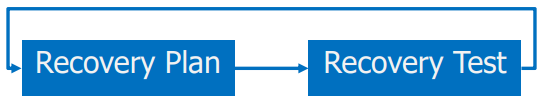
\includegraphics[width=0.7\linewidth]{recovery_plan_test.png}

    \textbf{Recovery Plan} - description of what to do if something goes wrong
    \begin{itemize}
        \item Roles and responsibilities
        \item Processes
        \item Contact details
        \item Technical instructions
    \end{itemize}

    \textbf{Recovery Test} - testing the recovery plan
    \begin{itemize}
        \item Theoretical dry run
        \item Practical tests
        \begin{itemize}
            \item turn off a server or DC
            \item restore data from backup
        \end{itemize}
    \end{itemize}
\end{formula}

\begin{concept}{Goals of IT Security}

Most measures in Information Security have one of the three following high-level goals:
\begin{itemize}
    \item Ensure data is confidential
    \item Ensure data is not corrupted
    \item Ensure data and systems are available
\end{itemize}

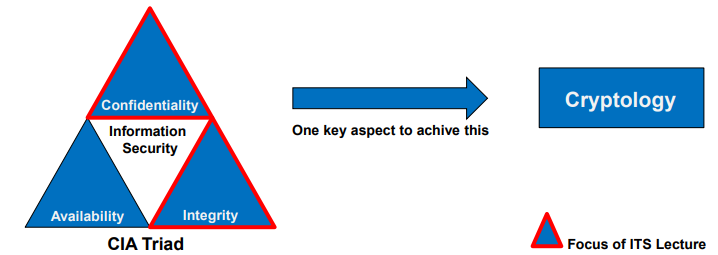
\includegraphics[width=\linewidth]{goals_of_IT_security.png}
\end{concept}

\multend

\raggedcolumns





	%\section{Computer Engineering}

\section*{Hardware}
\begin{itemize}
  \item CPU Central Processing Unit
  \item Memory Stores instructions and data
  \item Input / Output Interface to external devices
  \item System-Bus Electrical connection of blocks\\
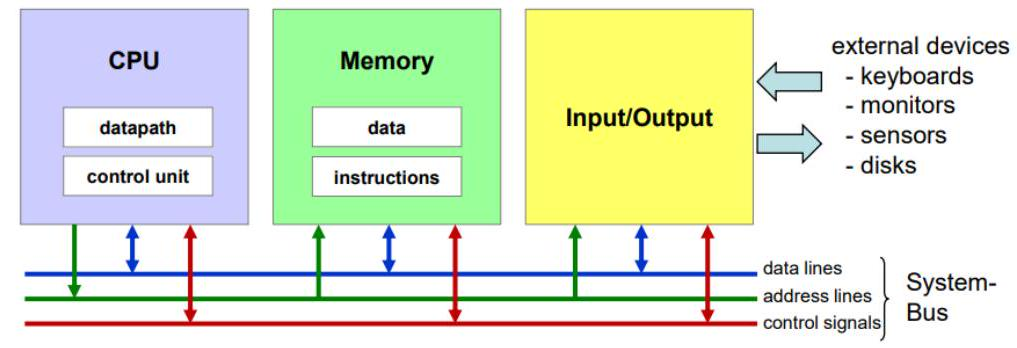
\includegraphics[max width=\textwidth, center]{2024_12_29_79e6b22f503fb7b4f718g-01(1)}
\end{itemize}

\section*{Datapath}
\begin{itemize}
  \item ALU
  \item Registers
\end{itemize}

Arithmetic and Logic Unit Fast but limited storage inside CPU

Control Unit

\begin{itemize}
  \item Finite State Machine
\end{itemize}

Reads and executes instructions

\begin{itemize}
  \item Types of instructions Data transfer, Arithemtic, logical and jumps
\end{itemize}

\section*{Software}
\section*{From C to executable}
\begin{center}
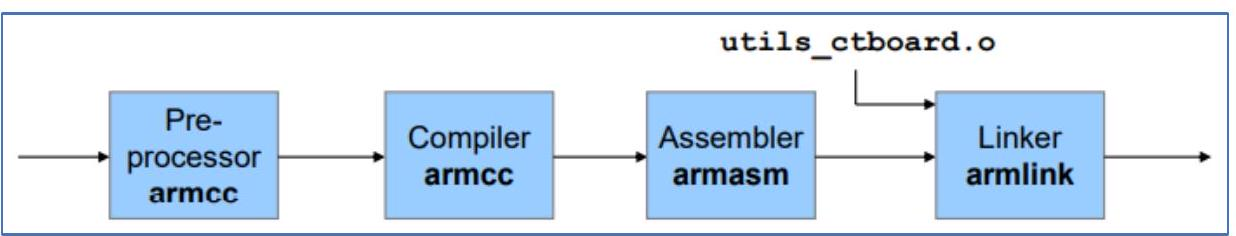
\includegraphics[max width=\textwidth]{2024_12_29_79e6b22f503fb7b4f718g-01}
\end{center}

\begin{enumerate}
  \item Preprocessor
\end{enumerate}

\begin{itemize}
  \item Text processing
  \item Pasting of \#include files
  \item Replacing macros (\#define)
\end{itemize}

\begin{enumerate}
  \setcounter{enumi}{1}
  \item Compiler
\end{enumerate}

\begin{itemize}
  \item Translate CPU-independent C-code into CPU-specific assembly code
\end{itemize}

\begin{enumerate}
  \setcounter{enumi}{2}
  \item Assembler
\end{enumerate}

\begin{itemize}
  \item Translate to machine instructions
  \item Result: Relocatable object file
  \item Binary file $\rightarrow$ not readable with text editor
\end{itemize}

\begin{enumerate}
  \setcounter{enumi}{3}
  \item Linker
\end{enumerate}

\begin{itemize}
  \item Merge object files
  \item Resolve dependencies and cross-references
  \item Create executable
\end{itemize}
	%\section{Cortex-M Architecture}

\section*{Registers}
\begin{itemize}
  \item 16 Core Registers
  \item 32-Bit wide
  \item RO-R7 Lower Registers
  \item R8 - R12 Higher Registers
  \item R13 Stack Pointer Temp Storage
  \item R14 Link Register Return from Procs
  \item R15 Program Counter Addr of next Instr.
\end{itemize}

\section*{ALU}
\begin{itemize}
  \item 32-Bit wide processing unit
\end{itemize}

\section*{APSR (Flag Register)}
\begin{itemize}
  \item N Negative
  \item Z Zero
  \item C Carry
  \item V Overflow
\end{itemize}

\section*{Instruction Set}
\begin{center}
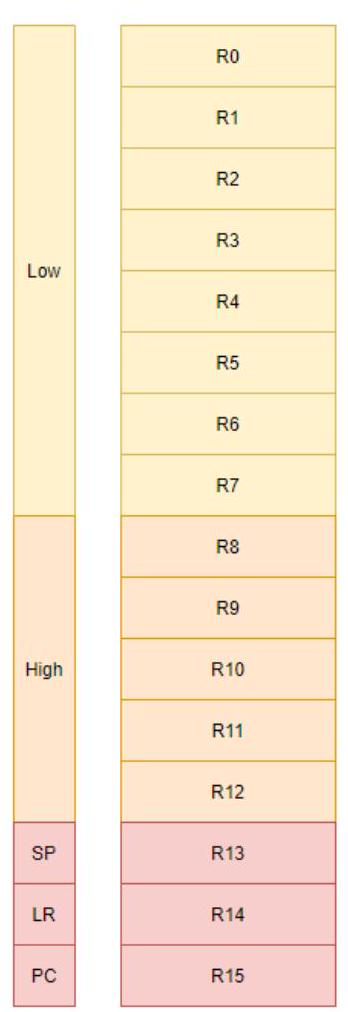
\includegraphics[width=\linewidth]{images/2024_12_29_79e6b22f503fb7b4f718g-02}
\end{center}

\begin{itemize}
  \item 16-Bit Thumb instruction encoding
\end{itemize}

\begin{center}
\begin{tabular}{llll}
Label & Instr. & Operands & Comments \\
\hline
demoprg & MOVS & R0,\#0xA5 & ; copy 0xA5 into register R0 \\
 & MOVS & R1,\#0x11 & ; copy 0x11 into register R1 \\
 & ADDS & R0,R0,R1 & ; add contents of RO and R1 \\
\end{tabular}
\end{center}

\section*{Instruction Types}
\begin{itemize}
  \item Data transfer
  \item Data processing
  \item Control flow Move, Load and Store\\
Arithmetic, Logical and Shift operations\\
Branches and functions
\end{itemize}

\section*{Assembly Program Structure}
\begin{center}
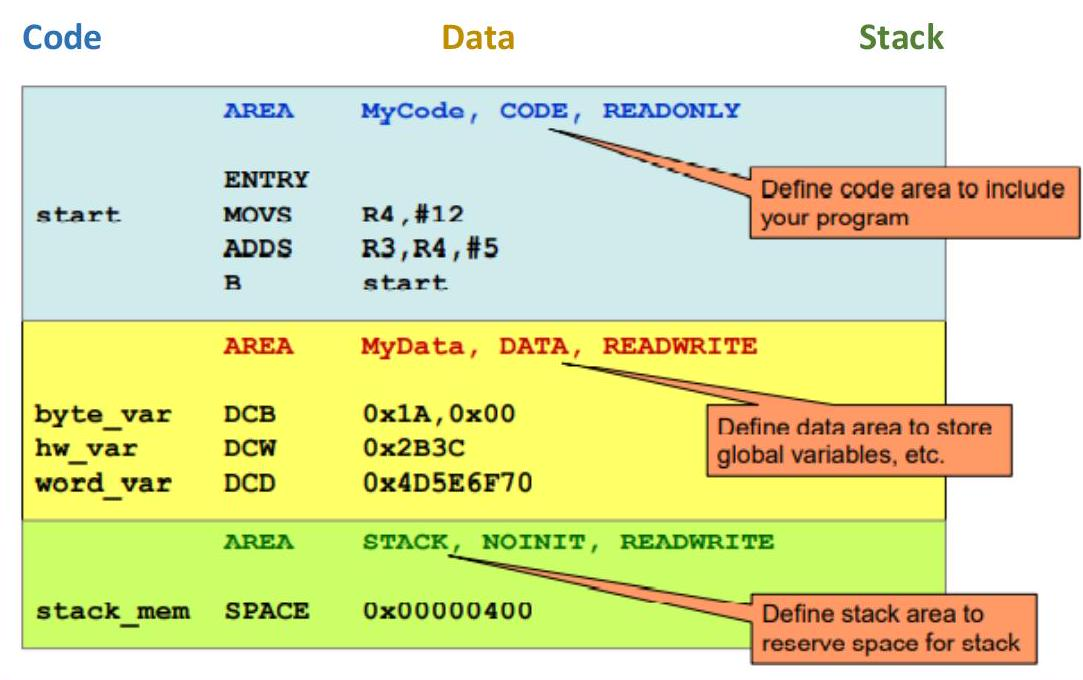
\includegraphics[width=\linewidth]{images/2024_12_29_79e6b22f503fb7b4f718g-02(1)}
\end{center}

Directives for initialized data

\begin{itemize}
  \item DCB Bytes
  \item DCW Half-Words
  \item DCD Words
\end{itemize}

\begin{center}
\begin{tabular}{|c|c|c|c|c|c|}
\hline
var1 & DCB & 0x1A &  &  &  \\
\hline
var2 & DCB & 0x2B & 0x3C & 0×4D & 0x5E \\
\hline
var3 & DCW & \multicolumn{2}{|r|}{0x6F70} & \multicolumn{2}{|c|}{0x8192} \\
\hline
var4 & $D C D$ & \multicolumn{4}{|c|}{0xA3B4C5D6} \\
\hline
\end{tabular}
\end{center}

Directives for uninitialized data

\begin{itemize}
  \item SPACE Bytes to be reserved
\end{itemize}
	%\section{Data Transfer}

\section*{Data Transfer Instructions}
\section*{Loading Data}
\begin{itemize}
  \item MOVS
  \item Reg to Reg MOVS R1, R2
  \item 8-Bit Literal MOVS R1,\#0x1C
  \item Constant MOVS R1, \#MyConst
  \item LDR
  \item 32-Bit Literal LDR R1, \#OxA1B2C3D4
  \item Literal + Offset LDR R1, [PC, \#12]
  \item Constant LDR R1, =MyConst
  \item Reg Value LDR R1, [R2]
  \item LDRB
  \item Load Register Byte
  \item Bits 31 to 8 set to zero
  \item LDRH
  \item Load Register Half-word
  \item Bits 31 to 16 set to zero
\end{itemize}

\section*{Load Array}
\begin{itemize}
  \item my\_array $=3$ * 4 Bytes
  \item Instructions $=5$ * 2 Bytes
  \item Literals (0x08) $=1 * 4$ Bytes\\
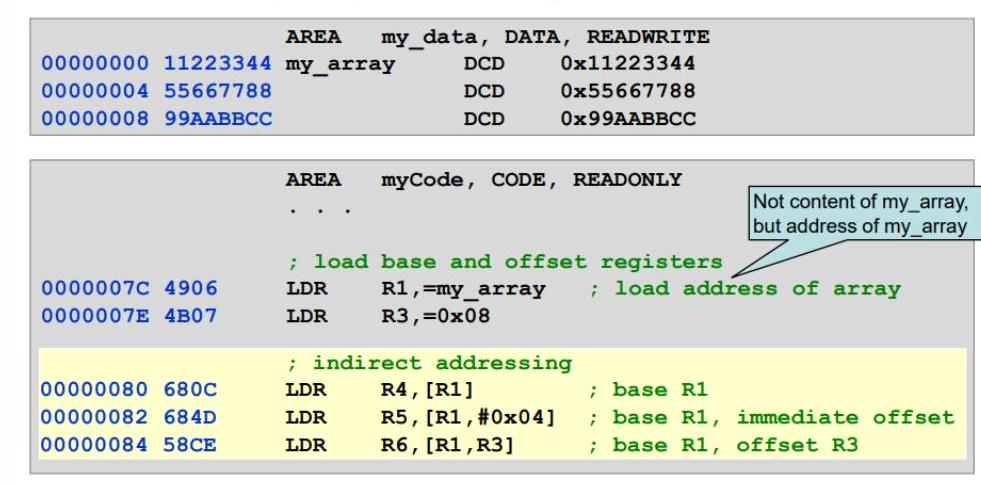
\includegraphics[max width=\textwidth, center]{2024_12_29_79e6b22f503fb7b4f718g-03(1)}\\
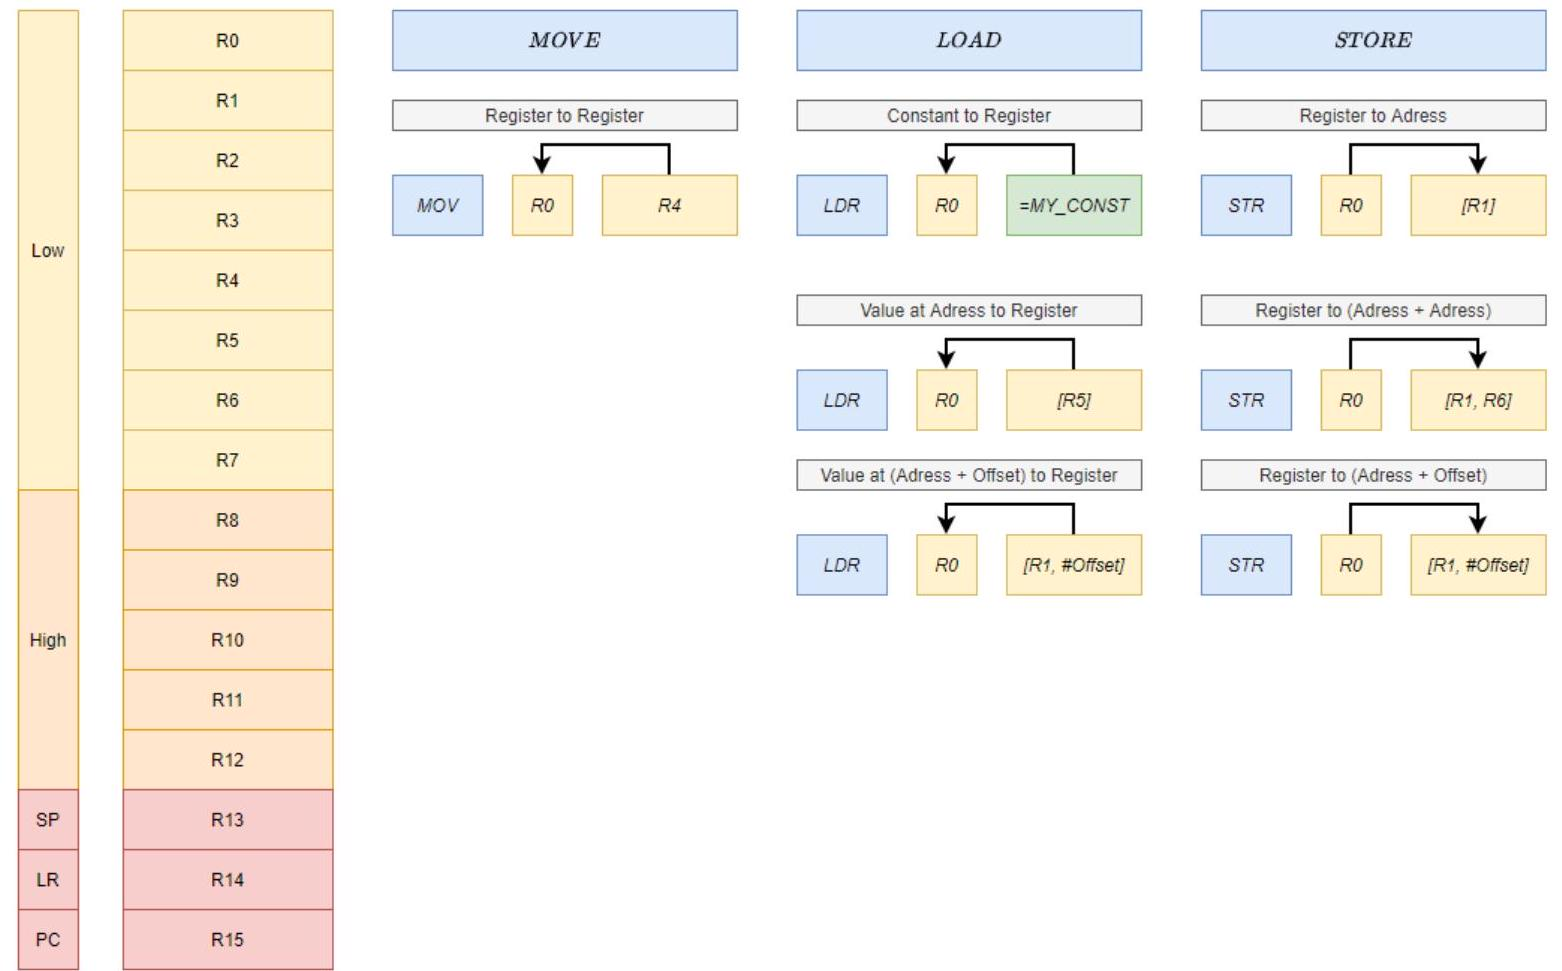
\includegraphics[max width=\textwidth, center]{2024_12_29_79e6b22f503fb7b4f718g-03}
\end{itemize}

Storing Data

\begin{itemize}
  \item STR
  \item Value from Register STR R1, [R2]
  \item Value from Reg + Offset $S T R R 1,[R 2, \# 0 x 04]$
  \item STRB
  \item Store Register Byte (Low 8 bits of register stored)
  \item STRH
  \item Store Register Half-word (Low 15 bits of register stored)
\end{itemize}
	%\section{Arithmetic Operations}

\section*{Arithmetic Operations}
Flags (APSR = N, Z, C, V)\\
Instructions ending with with «S» allow flag modification

\begin{itemize}
  \item ADDS
  \item SUBS
  \item MOVS
  \item LSLS
\end{itemize}

\begin{center}
\begin{tabular}{|llll|}
\hline
Flag & Meaning & Action & Operands \\
\hline
Negative & MSB =1 & $\mathrm{N}=1$ & signed \\
Zero & Result $=0$ & $\mathrm{Z}=1$ & signed, unsigned \\
Carry & Carry & $\mathrm{C}=1$ & unsigned \\
Overflow & Overflow & $\mathrm{V}=1$ & signed \\
\hline
\end{tabular}
\end{center}

\section*{Overview}
\begin{itemize}
  \item ADD / ADDS
  \item ADCS Addition with Carry
  \item ADR Address to Register
  \item SUB / SUBS
  \item SBCS
  \item RSBS
  \item MULS
\end{itemize}

Subtraction\\
Subtraction with carry (borrow)\\
Reverse Subtract (negative)\\
Multiplication\\
$A+B$\\
$A+B+c$\\
$P C+A$\\
$A-B$\\
$A-B-!c$\\
$-1 \cdot A$\\
$A \cdot B$

Multi-Word Addition with ADCS\\
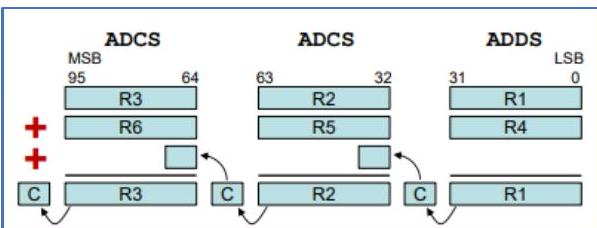
\includegraphics[max width=\textwidth, center]{2024_12_29_79e6b22f503fb7b4f718g-04}

\begin{center}
\begin{tabular}{|c|c|c|c|}
\hline
ADDS & R1, & R1, & R4 \\
\hline
ADCS & R2, & R2, & R5 \\
\hline
ADCS & R3, & R3, & R6 \\
\hline
\end{tabular}
\end{center}

Multi-Word Subtraction with SBCS\\
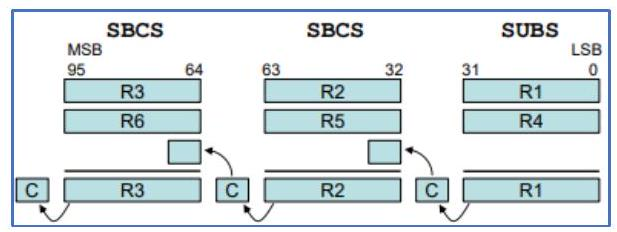
\includegraphics[max width=\textwidth, center]{2024_12_29_79e6b22f503fb7b4f718g-04(1)}

\begin{center}
\begin{tabular}{|c|c|c|c|}
\hline
SUBS & R1, & R1, & R4 \\
\hline
SBCS & R2, & R2, & R5 \\
\hline
SBCS & R3, & R3, & R6 \\
\hline
\end{tabular}
\end{center}

\section*{Negative Number}
\begin{itemize}
  \item 2' Complement $\quad A=!A+1$
\end{itemize}

\section*{Carry and Overflow}
unsigned

\begin{itemize}
  \item Addition $\rightarrow \quad \mathrm{C}=1 \rightarrow$ carry result too large for available bits
  \item Subtraction $\rightarrow \mathrm{C}=0 \rightarrow$ borrow result less than zero $\rightarrow$ no negative numbers\\
signed
  \item Addition $\rightarrow \quad$ potential overflow in case of operands with equal signs
  \item Subtraction $\rightarrow$ potential overflow in case of operands with opposite signs
\end{itemize}

\section*{Addition and Subtraction}
\begin{itemize}
  \item Addition $\quad \mathrm{C}=1 \rightarrow$ Carry
\end{itemize}

\begin{center}
\begin{tabular}{|rrrrr|}
\hline
1 & 1 & 0 & 1 & $13 d$ \\
0 & 1 & 1 & 1 & $7 d$ \\
1 & 1 & 1 & 1 &  \\
1 &  &  &  &  \\
1 & 0 & 1 & 0 & 0 \\
\end{tabular}
\end{center}

\begin{itemize}
  \item Subtraction $\quad \mathrm{C}=0 \rightarrow$ Borrow sign\\
$6 d-14 d=0110 b-1110 b=0110 b+0010 b$
\end{itemize}

$$
\begin{array}{llllll}
0 & 1 & 1 & 0 & 6 d \\
0 & 0 & 1 & 0 & 2 d=\operatorname{TC}(14 d)
\end{array}
$$

0100\\
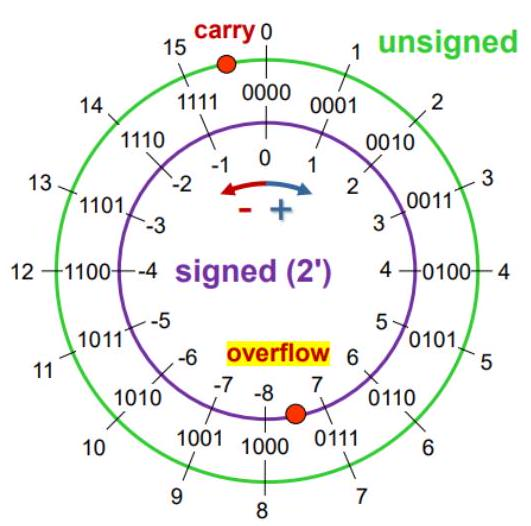
\includegraphics[max width=\textwidth, center]{2024_12_29_79e6b22f503fb7b4f718g-04(2)}

	%\section{Logic, Shift and Rotate Instructions}

\section*{Logical Instructions}
The following instruction only affect N and Z flags

\begin{itemize}
  \item ANDS
  \item BICS
  \item EORS
  \item MVNS Bitwise NOT
  \item ORRS
\end{itemize}

Bitwise OR

Rdn \# Rm\\
Rdn \& Rm\\
Rdn \& ! Rm $\quad a \& \sim b$\\
Rdn \$ Rm $\quad a{ }^{\wedge} b$\\
Rm a\\
a | b

Shift Instructions

\begin{itemize}
  \item LSLS Logical Shift Left $\quad 2^{n} \cdot R n \quad 0 \rightarrow L S B$
  \item LSRS Logical Shift Right $\quad 2^{-n} \cdot R n \quad 0 \rightarrow M S B$
  \item ASRS Arithmetic Shift Right $\quad R^{-n} \pm \pm M S B \rightarrow M S B$
  \item RORS Rotate Right $\quad L S B \rightarrow M S B$\\
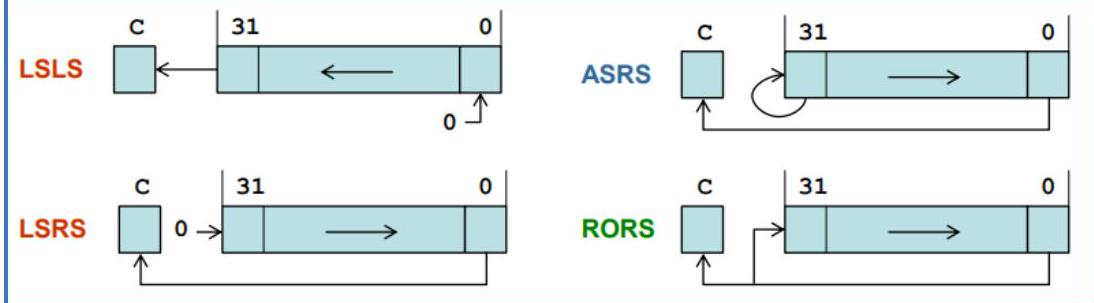
\includegraphics[max width=\textwidth, center]{2024_12_29_79e6b22f503fb7b4f718g-06}
\end{itemize}

\section*{Sign-Extension}
Add additional bits

\begin{itemize}
  \item Unsigned zero extension fill left bits with zero
  \item Signed sign extension copy sign bit to the left
\end{itemize}

\begin{center}
\begin{tabular}{|c|c|c|c|c|}
\hline
\multicolumn{2}{|l|}{Unsigned $\rightarrow \boldsymbol{\sim}$ Zero Extension} &  & \multirow[b]{2}{*}{$\rightarrow$} & \multirow[b]{2}{*}{00000011} \\
\hline
$1011 \rightarrow$ & 00001011 & 0011 &  &  \\
\hline
\multicolumn{5}{|l|}{Signed $\boldsymbol{\rightarrow}$ Sign Extension} \\
\hline
$1011 \rightarrow$ & 11111011 & 0011 & $\rightarrow$ & 00000011 \\
\hline
\end{tabular}
\end{center}

\section*{Truncation}
Cast cuts out the left most digits

\begin{itemize}
  \item Signed possible change of sign
  \item Unsigned results in module operation
\end{itemize}

\section*{Integer ranges based on word sizes}
\begin{center}
\begin{tabular}{|c|c|c|c|c|c|c|c|}
\hline
\multirow[t]{6}{*}{8-bit} & \( \begin{gathered} \text { hex } \\ 0 \times 00 \end{gathered} \) & unsigned & signed & 16-bit & hex 0×0000 & unsigned & signed \\
\hline
 &  &  &  &  &  &  &  \\
\hline
 & 0x75 & 127 & 127 &  & 0x7FFF & F 32'767 & $32 \cdot 767$ \\
\hline
 & 0x80 & 128 & -128 &  & 0x8000 & $032 \cdot 768$ & -32'768 \\
\hline
 &  & . . . & -. &  & . . & . . &  \\
\hline
 & 0xFF & 255 & -1 &  & 0xFFFF & F 65'535 & -1 \\
\hline
\multicolumn{2}{|r|}{\multirow[t]{7}{*}{32-bit}} & \multicolumn{2}{|l|}{hex} & \multicolumn{2}{|l|}{unsigned} & signed &  \\
\hline
 &  & \multicolumn{2}{|l|}{0x0000 0000} & \multicolumn{2}{|l|}{o} & 0 &  \\
\hline
 &  & \multicolumn{2}{|l|}{\multirow[t]{2}{*}{0x7FFF'FFFF}} & \multicolumn{2}{|l|}{\multirow[t]{2}{*}{2'147'483'647}} & ... &  \\
\hline
 &  &  &  &  &  & 2'147'483' &  \\
\hline
 &  & \multicolumn{2}{|l|}{0x8000'0000} & \multicolumn{2}{|l|}{2'147'483'648 -} & -2'147'483' &  \\
\hline
 &  & \multicolumn{2}{|l|}{\multirow[t]{2}{*}{0xFFFF'FFFF}} & \multicolumn{2}{|l|}{\multirow[t]{2}{*}{4'294'967'295}} & -. &  \\
\hline
 &  &  &  &  &  & -1 &  \\
\hline
\end{tabular}
\end{center}
	%\section{Control Structures}

%didn't work at all, write by hand
\section*{Branch Instructions}
\begin{center}
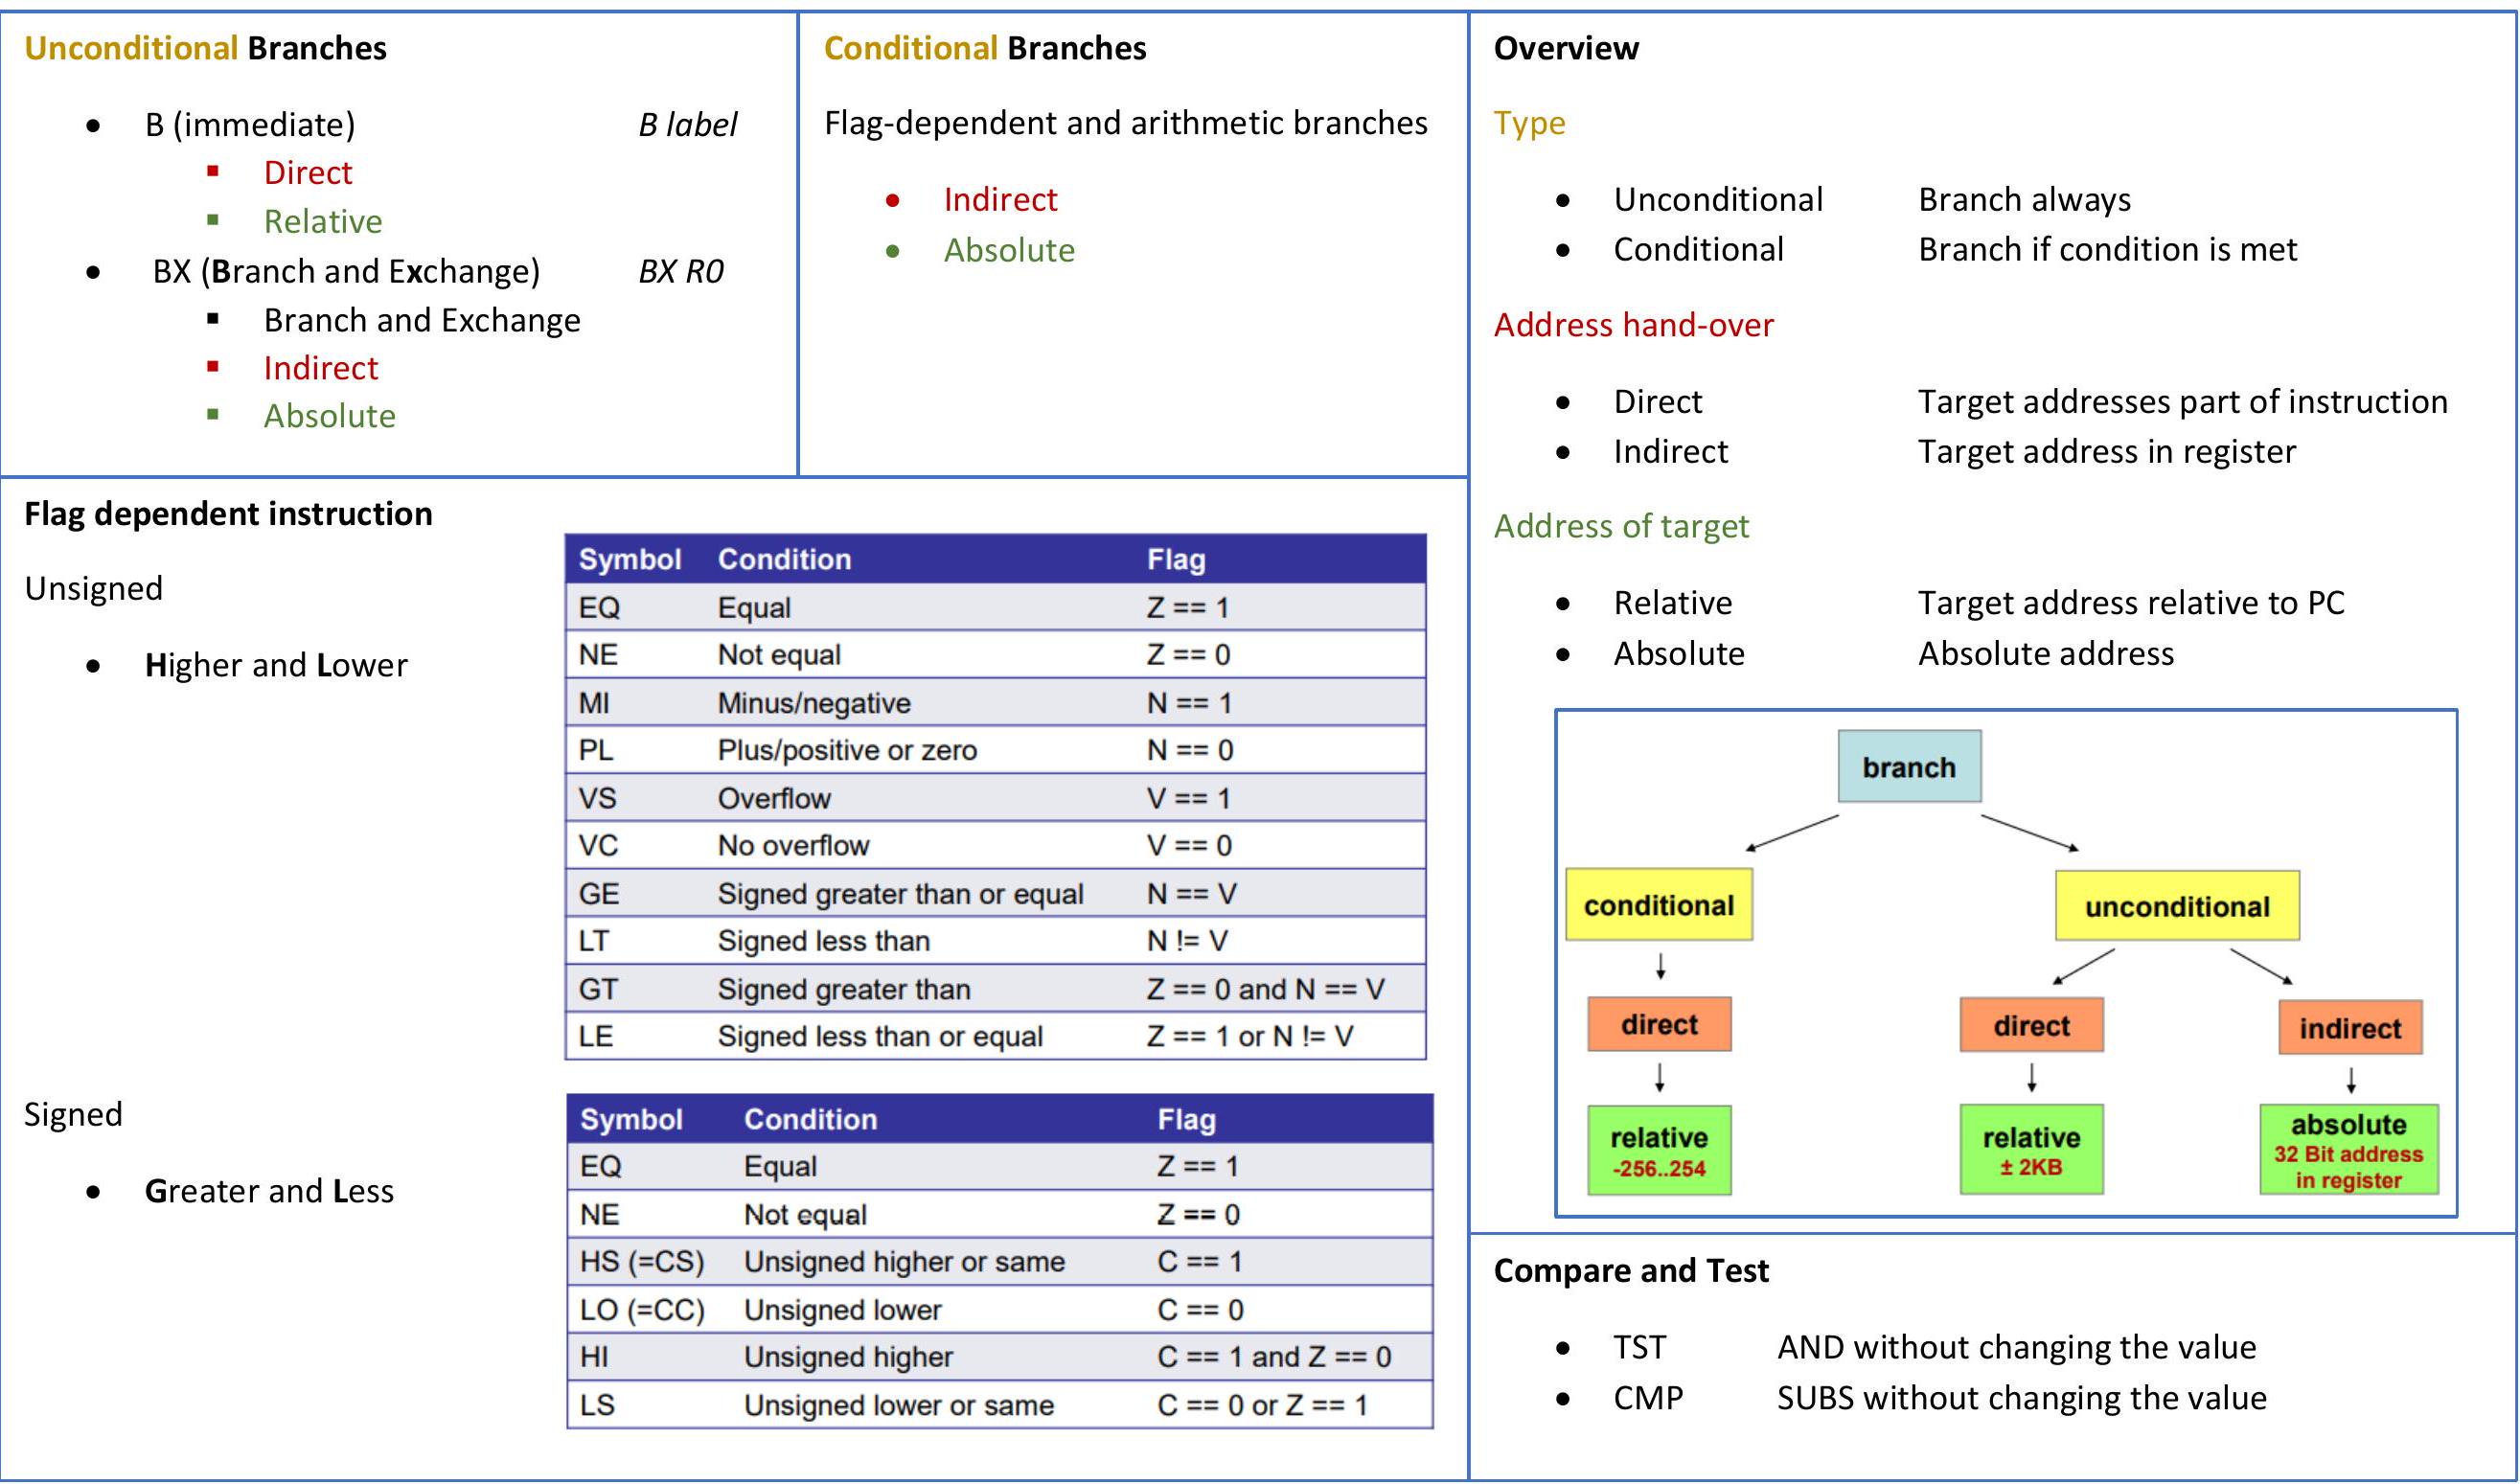
\includegraphics[max width=\textwidth]{2024_12_29_79e6b22f503fb7b4f718g-05}
\end{center}

\begin{center}
    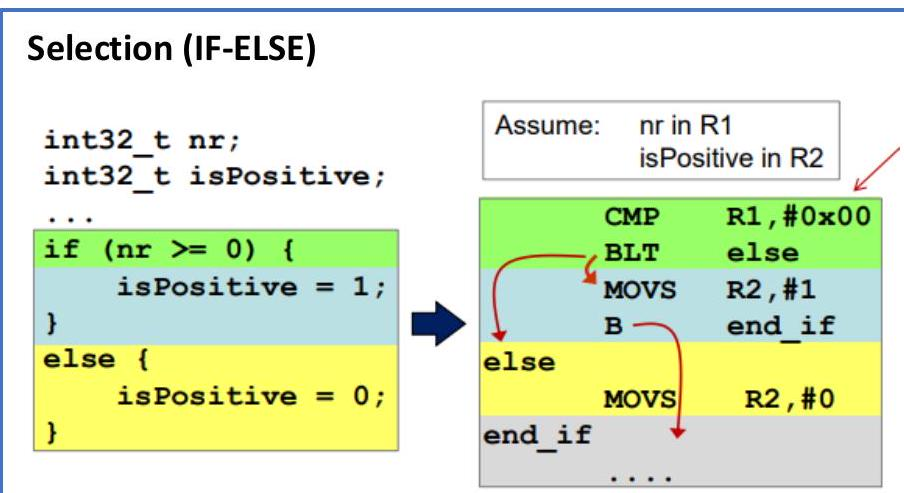
\includegraphics[max width=\textwidth]{2024_12_29_79e6b22f503fb7b4f718g-07(3)}
    \end{center}
    
    \section*{Switch}
    \section*{- Jump Table}
    uint32\_t result, n; switch (n) 1\\
    case 0:\\
    result += 17; break;\\
    case 1:\\
    result += 13; //fall through\\
    case 3: case 5 result += 37; break;\\
    default:\\
    result $=0$;\\
    \}
    
    \begin{center}
    \begin{tabular}{|c|c|c|}
    \hline
    \multirow[t]{7}{*}{NR\_CASES case\_switch} & EQU & 6 \\
    \hline
     & CMP & R1, \#NR\_CASES \\
    \hline
     & BHS & case\_default \\
    \hline
     & LSLS & R1, \#2 ; * 4 \\
    \hline
     & LDR & R7, =jump\_table \\
    \hline
     & LDR & R7, [R7, R1] \\
    \hline
     & BX & R7 \\
    \hline
    case\_0 & ADDS & R2, R2, \#17 \\
    \hline
    case\_1 & ADDS & R2, R2, \#13 \\
    \hline
    \multirow[t]{2}{*}{case\_3\_5} & ADDS & R2, R2, \#37 \\
    \hline
     & B & end\_sw\_case \\
    \hline
    case\_default & Movs & R2,\#0 \\
    \hline
    end\_sw\_case & ... &  \\
    \hline
    \multirow[t]{6}{*}{jump\_table} & DCD & case\_0 \\
    \hline
     & DCD & case\_1 \\
    \hline
     & DCD & case\_default \\
    \hline
     & DCD & case\_3\_5 \\
    \hline
     & DCD & case\_default \\
    \hline
     & DCD & case\_3\_5 \\
    \hline
    \end{tabular}
    \end{center}
    
    \section*{Loops}
    \begin{itemize}
      \item Do while: Post-Test Loop\\
    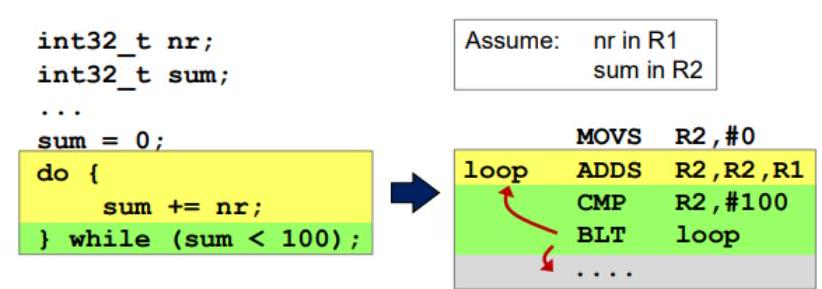
\includegraphics[max width=\textwidth, center]{2024_12_29_79e6b22f503fb7b4f718g-07}
      \item While = Pre-Test Loop\\
    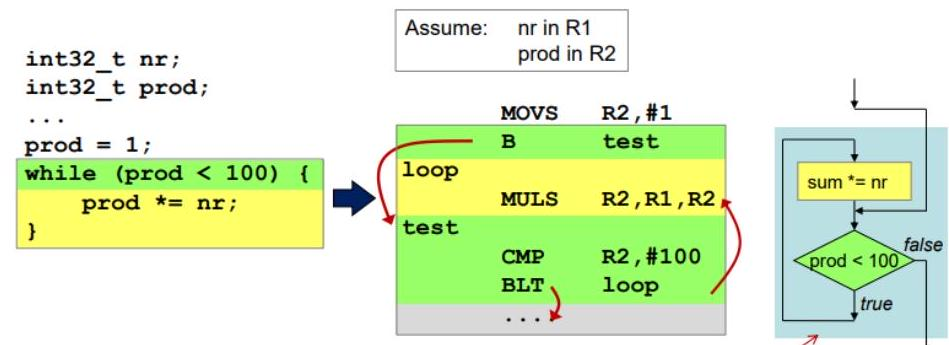
\includegraphics[max width=\textwidth, center]{2024_12_29_79e6b22f503fb7b4f718g-07(1)}
      \item For = Pre-Test Loop\\
    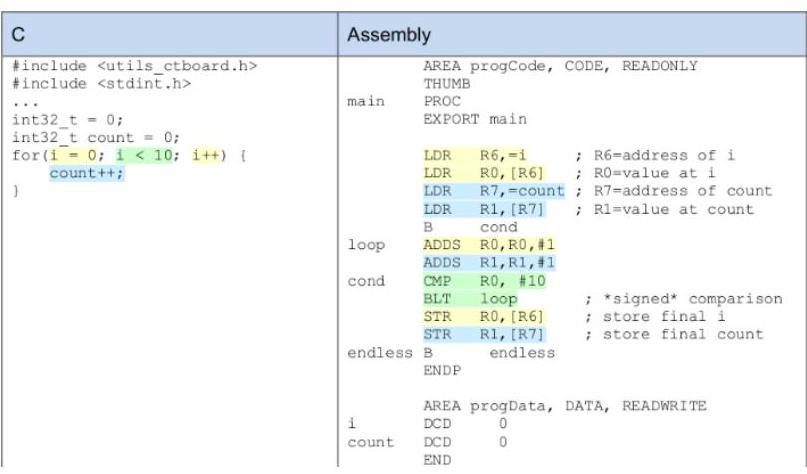
\includegraphics[max width=\textwidth, center]{2024_12_29_79e6b22f503fb7b4f718g-07(2)}
    \end{itemize}
	%\section{Subroutines and the Stack}
	%\section{Parameter Passing}

\section*{Where}
\begin{itemize}
  \item Register
  \item Global variables
  \item Stack
  \item Caller: PUSH parameter on stack
  \item Callee: Access parameter through LDR
\end{itemize}

\section*{Reentrancy}
\begin{itemize}
  \item Recursive Function Calls
  \item Registers and gobal variables are overwritten
  \item Requires an own set of data for each call
  \item Solution:
  \item ARM Procedure Call Standard
\end{itemize}

\section*{Passing through global variables}
\begin{itemize}
  \item Shared variables in data area
  \item Overhead to access variable
  \item Error prone, unmaintainable
  \item By reference
  \item Allows passing of larger structures
\end{itemize}

\section*{ARM Procedure call Standard}
\section*{Parameters}
\begin{itemize}
  \item Caller copies arguments From R0 to R3
  \item Caller copies additional parameters to stack
\end{itemize}

Returning fundamental data types

\begin{itemize}
  \item Smaller than word
  \item Word
  \item Double word
  \item 128-Bit\\
zero or sign extend to word return in RO return in RO / R1 return in RO - R3
\end{itemize}

Returning composite data types

\begin{itemize}
  \item Up to 4 bytes\\
return in RO
  \item Larger than 4 bytes stored in data area\\
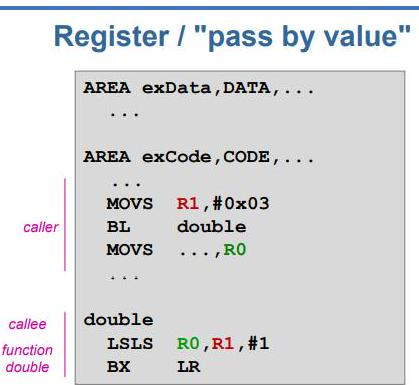
\includegraphics[width=\linewidth]{images/2024_12_29_79e6b22f503fb7b4f718g-09(2)}
\end{itemize}

Register Usage

\begin{center}
\begin{tabular}{|c|c|c|}
\hline
Register & Synonym & Role \\
\hline
ro & a1 & Argument / result / scratch register 1 \\
\hline
r1 & a2 & Argument / result / scratch register 2 \\
\hline
I2 & a3 & Argument / scratch register 3 \\
\hline
r3 & a4 & Argument / scratch register 4 \\
\hline
4$\tau$ & v1 & Variable register 1 \\
\hline
r5 & v2 & Variable register 2 \\
\hline
r6 & v3 & Variable register 3 \\
\hline
r7 & v4 & Variable register 4 \\
\hline
8$\tau$ & v5 & Variable register 5 \\
\hline
r9 & v6 & 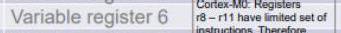
\includegraphics[width=\linewidth]{images/2024_12_29_79e6b22f503fb7b4f718g-09}
 \\
\hline
r10 & v7 & 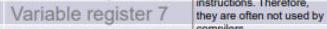
\includegraphics[width=\linewidth]{images/2024_12_29_79e6b22f503fb7b4f718g-09(1)}
 \\
\hline
r11 & v8 & Variable register 8 \\
\hline
r12 & IP & Intra-Procedure-call scratch register1) \\
\hline
r13 & SP &  \\
\hline
r14 & LR &  \\
\hline
\end{tabular}
\end{center}

Register contents\\
might be modified\\
might be modified

Callee must preserve contents\\
of these registers (Callee saved)\\
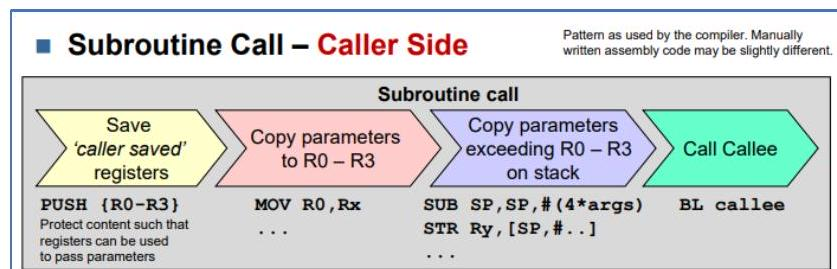
\includegraphics[width=\linewidth]{images/2024_12_29_79e6b22f503fb7b4f718g-09(3)}

On return from subroutine
	%\section{Modular Coding and Linking}

\section*{Modular Coding / Linking}
\section*{From source code to executable program}
Compile / assemble each module

\begin{itemize}
  \item Results in an object file for each module
\end{itemize}

Link all object files

\begin{itemize}
  \item Results in one executable file\\
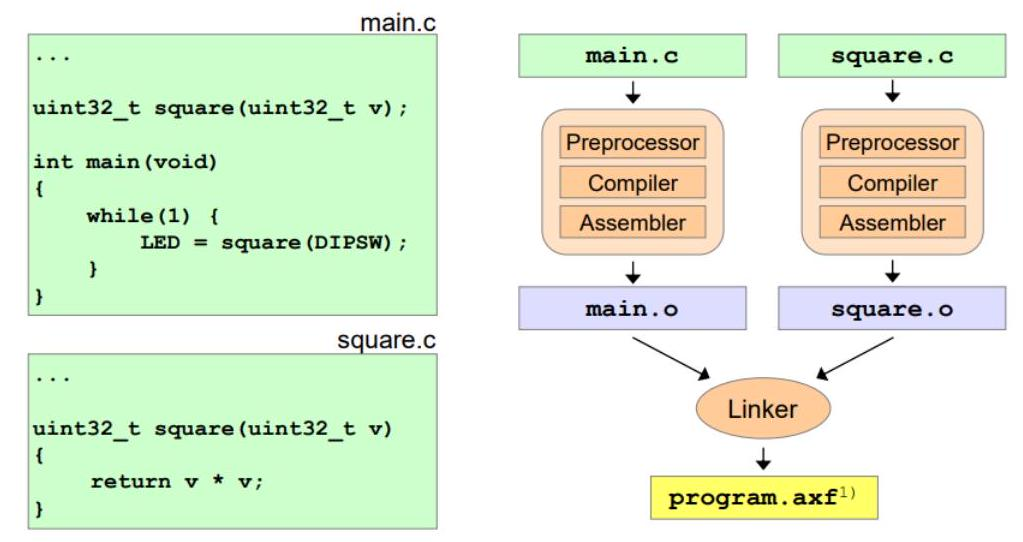
\includegraphics[max width=\textwidth, center]{2024_12_29_79e6b22f503fb7b4f718g-10(2)}
\end{itemize}

\section*{Managing complexity by modular programming}
\begin{center}
\begin{tabular}{|l|l|}
\hline
Topic & Benefits \\
\hline
Enable working in teams & \begin{tabular}{l}
Multiple developers working on the same source \\
repository \\
\end{tabular} \\
\hline
Useful partitioning and structuring of the programs & Eases reuseing of modules \\
\hline
Individual verification of each module & Benefits all users of the module \\
\hline
Providing libraries of types and functions & For reuse instead of reinvention \\
\hline
\begin{tabular}{l}
Mixing of modules that are programmed in various \\
languages \\
\end{tabular} & E.g. mix C and assembly language modules \\
\hline
Only compile the changed modules & Speeds up compilation time \\
\hline
\end{tabular}
\end{center}

\section*{ARM assembly IMPORT and EXPORT keywords}
Linkage control

\begin{itemize}
  \item EXPORT for use by other module
  \item IMPORT from another module for use in this module Internal symbols
  \item Neither IMPORT nor EXPORT\\
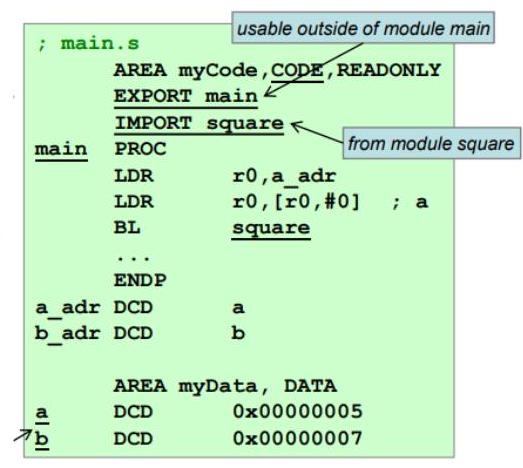
\includegraphics[max width=\textwidth, center]{2024_12_29_79e6b22f503fb7b4f718g-10(1)}
\end{itemize}

\section*{Linker Input - Object files}
Code section Code and constant data of the module, base at address $0 \times 0$\\
Data section All global variables of the module, based at address $0 \times 0$\\
Symbol table All symbols with their attributes like global/local, reference\\
Relocation table

\begin{itemize}
  \item Which bytes oft he data and code section need to be adjusted (and how) after merging the sections in the linking process
\end{itemize}

ARM tool chain uses ELF for object files

\section*{Linker tasks}
\begin{itemize}
  \item Merge object file code sections
  \item Merge object file data sections
  \item Symbol resolution
  \item Address relocation
\end{itemize}

\section*{Linker Output}
\begin{itemize}
  \item $\quad$ AXF $=\mathbf{A R M}$ eXecutable File\\
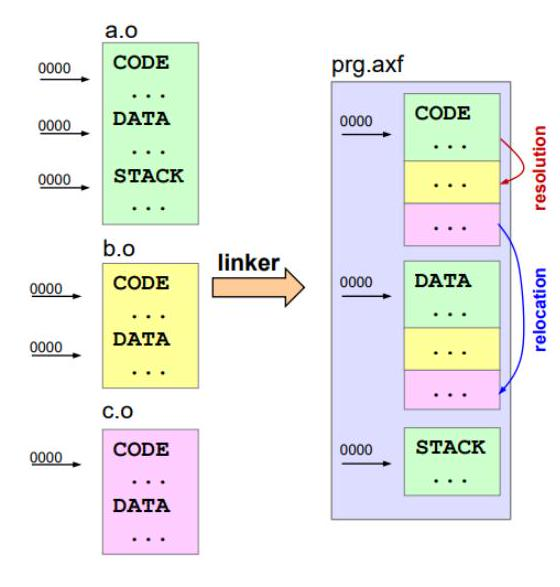
\includegraphics[max width=\textwidth, center]{2024_12_29_79e6b22f503fb7b4f718g-10}
\end{itemize}
	%\section{Exceptional Control Flow}
	%\section{Increasing System Performance}

\begin{center}
    \begin{tabular}{|l|l|}
    \hline
    Speed vs Low Power &  \\
    Aspects of Optimization &  \\
    \hline
    Optimizing for & Drawbacks on \\
    \hline
    Higher speed & Power, cost, chip area \\
    \hline
    Lower cost & Speed, reliability \\
    \hline
    Zero power consumption & Speed, cost \\
    \hline
    Super reliable & Chip area, cost, speed \\
    \hline
    Temperature range & Power, cost lifetime \\
    \hline
    \end{tabular}
    \end{center}
    
    \section*{RISC = Reduced Instruction Set Computer}
    \begin{itemize}
      \item Few instructions, unique instruction format
      \item Fast decoding, simple addressing
      \item Less hardware -> allows higher clock rates
      \item More chip space for registers (up to 256!)
      \item Load-store architecture reduces memory access,
    \end{itemize}
    
    CPU works at full-speed on registers
    
    \begin{itemize}
      \item Higher clock frequencies
      \item Easy and shorter pipelines (instructio size / duration)\\
    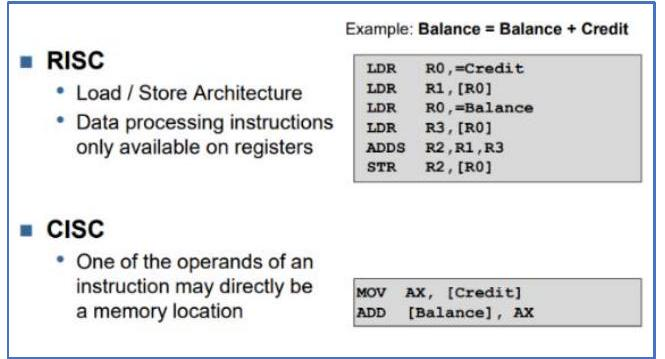
\includegraphics[width=\linewidth]{images/2024_12_29_79e6b22f503fb7b4f718g-13(1)}
    \end{itemize}
    
    CISC = Complex Instruction Set Computer
    
    \begin{itemize}
      \item More complex and more instructions
      \item Less program memory needed with complex instructions
      \item Short programs may work faster with less memory accesses
    \end{itemize}
    
    \section*{Von Neuman Arhcitecture}
    \begin{itemize}
      \item Same memory holds program and data
      \item $\quad$ Single bus system between CPU and memory Systembus\\
    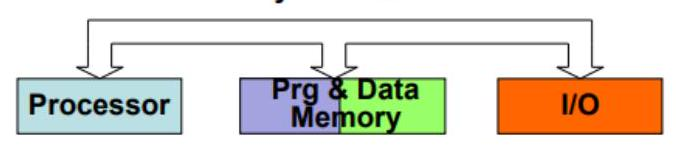
\includegraphics[width=\linewidth]{images/2024_12_29_79e6b22f503fb7b4f718g-13}
    \end{itemize}
    
    \section*{Harvard Architecture}
    \begin{itemize}
      \item «Mark I» at Harvard University
      \item Separate memories for program and data
      \item Two sets of addresses/data buses between CPU and memory\\
    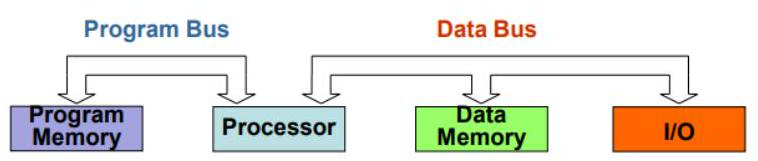
\includegraphics[width=\linewidth]{images/2024_12_29_79e6b22f503fb7b4f718g-13(2)}
    \end{itemize}
    
    How to Increase System Speed?\\
    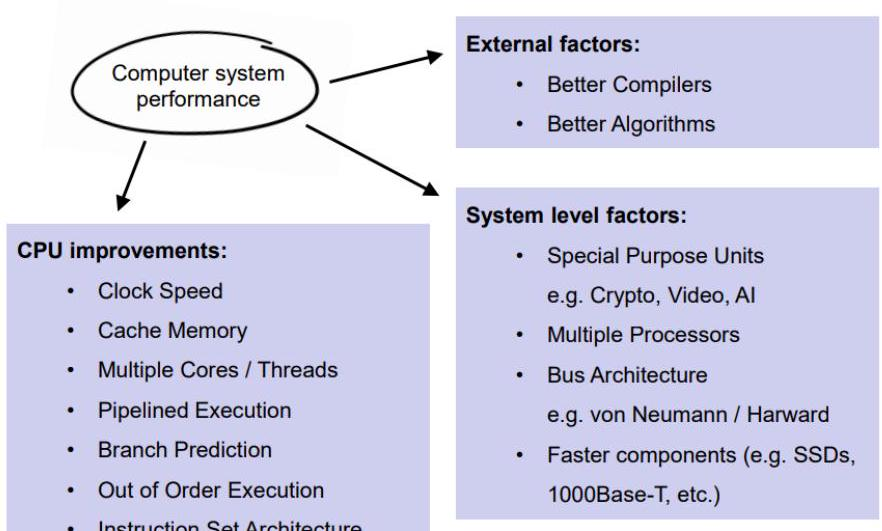
\includegraphics[width=\linewidth]{images/2024_12_29_79e6b22f503fb7b4f718g-13(3)}
    
    Fetching the next instruction, while the current one decodes\\
    Sequential vs. Pipelined\\
    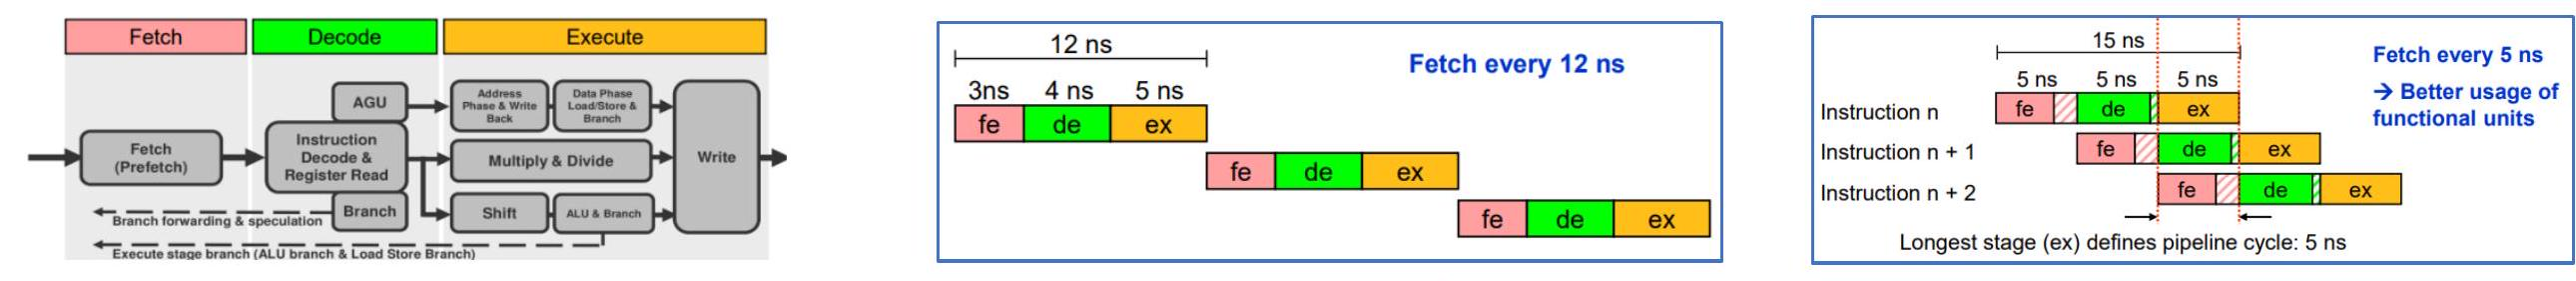
\includegraphics[width=\linewidth]{images/2024_12_29_79e6b22f503fb7b4f718g-14(2)}
    
    \section*{Timings and definitions (Example)}
    \begin{itemize}
      \item Fe: fetch Read instructions 3 ns
      \item De: decode Decode instruction, read register or memory 4 ns
      \item Ex: execute Execute instruction, write back result 5 ns\\
    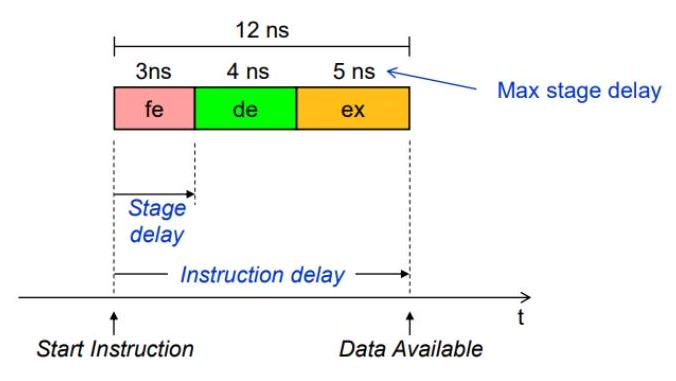
\includegraphics[width=\linewidth]{images/2024_12_29_79e6b22f503fb7b4f718g-14(1)}
    \end{itemize}
    
    \section*{Advantages of pipelining}
    \begin{itemize}
      \item All stages are set tot he same execution time
      \item Massive performance gain
      \item Simpler hardware at each stage allows for a higher clock rate
    \end{itemize}
    
    \section*{Disadvantages}
    \begin{itemize}
      \item A blocking stage blocks while pipeline
      \item Multiple stages may need to have access to the memory at the same time
    \end{itemize}
    
    \section*{Instructions per second}
    Without pipelining
    
    $$
    \frac{\text { Instructions }}{\text { second }}=\frac{1}{\text { Instruction delay }}
    $$
    
    With pipelining
    
    \begin{itemize}
      \item Pipeline needs to be filled first
      \item After filling, instructions are executed after every stage
    \end{itemize}
    
    $$
    \frac{\text { Instructions }}{\text { second }}=\frac{1}{\text { Max stage delay }}
    $$
    
    \section*{Optimal pipelining}
    \begin{itemize}
      \item All operations here are on registers
      \item In this example it takes 6 clock cycles to execute 6 instructions
      \item $\quad$ Clock cycles per instruction (CPI) = 1\\
    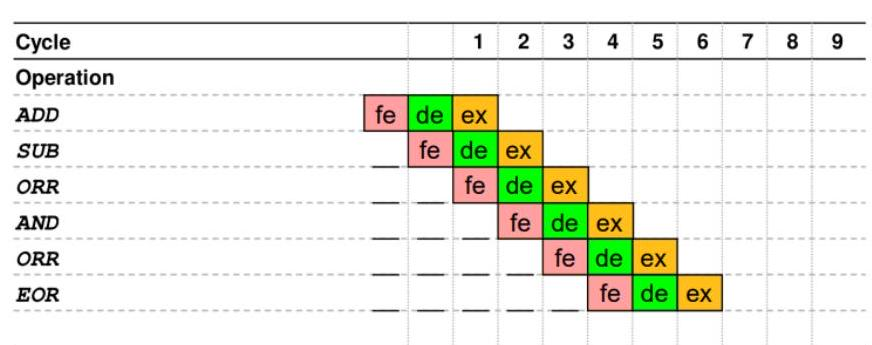
\includegraphics[width=\linewidth]{images/2024_12_29_79e6b22f503fb7b4f718g-14}
    \end{itemize}
    
    \section*{Special situation: LDR}
    \begin{itemize}
      \item In this example it takes 7 clock cycles to execute 6 instructions
      \item Read cycle must complete on the bus before LDR instruction can complete
      \item Next 2 instructions must wait one pipeline cycle ( $\mathrm{S}=$ stall)
      \item Clock cycles per Instruction (CPI) $=1.2$
    \end{itemize}
    
    \section*{Control Hazards}
    \begin{itemize}
      \item Branch / jump decisions occur in stage 3 (ex)
      \item Worst case scenario - conditional branch taken:\\
    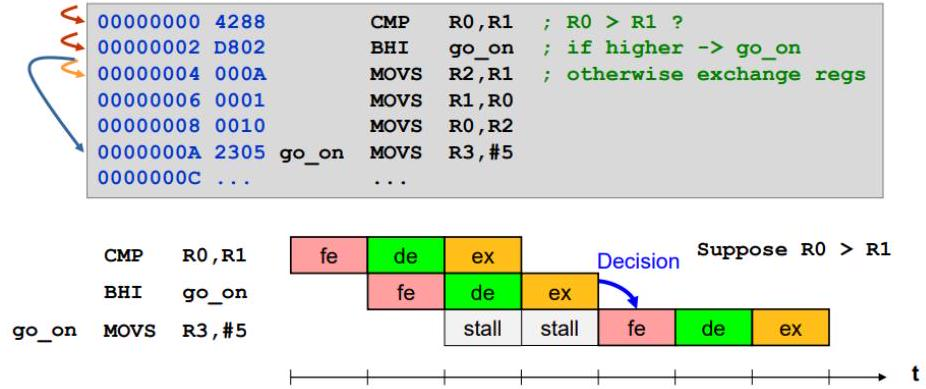
\includegraphics[width=\linewidth]{images/2024_12_29_79e6b22f503fb7b4f718g-15}
    \end{itemize}
    
    \section*{Reduce control hazards}
    \begin{itemize}
      \item Loop fusion reduces control hazards
    \end{itemize}
    
    \section*{Ideas to further improve pipelining}
    \begin{itemize}
      \item Branch prediction
      \item Store last decisions made for each conditional branch
      \item -> probability is high that the same decision is taken again
      \item Instruction prefetch
      \item Fetch several instructions in advance
      \item -> better use of system bus
      \item -> possibility of «Out of Order Execution»
      \item Out of Order Execution
      \item If one instruction stalls, it might be possible to already execute the next instruction
    \end{itemize}
    
    \section*{Limits of optimization}
    \begin{itemize}
      \item Complex optimizations -> sever security problems
      \item Instructions executed, that would throw access violations under «In Order» circumstances.
      \item «Meltdown» and «Spectre» attacks: allow a process to access the data of another process
    \end{itemize}
    
    \section*{Parallel Computing}
    \begin{itemize}
      \item Streaming / Vector processing One instruction processes multiple data items simultaneously
      \item Multithreading Multiple programs/threads share a single CPU
      \item Multicore Processors One processor contains multiple CPU cores
      \item Multiprocessor Systems A computer system contains multiple processors
    \end{itemize}
	\raggedcolumns
	\pagebreak
	\section{Additional Examples}

\subsection{Rechnerarithmetik}

\begin{example2}{Werteberechnung ausführlich} 
Gegeben sei die Maschinenzahl zur Basis $B=2$:
$$x = \underbrace{0.1101}_{\text{n=4}} \cdot \underbrace{2^{101}_2}_{\text{l=3}}$$

\textbf{1. Normalisierung prüfen:}
\begin{itemize}
    \item $m_1 = 1 \neq 0$ $\rightarrow$ normalisiert
\end{itemize}

\textbf{2. Exponent berechnen:}
\begin{align*}
\hat{e} &= 1 \cdot 2^2 + 0 \cdot 2^1 + 1 \cdot 2^0 \\
&= 4 + 0 + 1 = 5
\end{align*}

\textbf{3. Wert berechnen:}
\begin{align*}
\hat{\omega} &= 1 \cdot 2^{5-1} + 1 \cdot 2^{5-2} + 0 \cdot 2^{5-3} + 1 \cdot 2^{5-4} \\
&= 1 \cdot 2^4 + 1 \cdot 2^3 + 0 \cdot 2^2 + 1 \cdot 2^1 \\
&= 16 + 8 + 0 + 2 \\
&= 26
\end{align*}

Also ist $x = 26$
\end{example2}

\begin{example2}{Weitere Beispiele}
\begin{enumerate}
    \item Basis 10: $0.3141 \cdot 10^2$
    \begin{itemize}
        \item Normalisiert, da $m_1 = 3 \neq 0$
        \item $\hat{e} = 2$
        \item $\hat{\omega} = 3 \cdot 10^1 + 1 \cdot 10^0 + 4 \cdot 10^{-1} + 1 \cdot 10^{-2} = 31.41$
    \end{itemize}
    
    \item Basis 16 (hex): $0.A5F \cdot 16^3$
    \begin{itemize}
        \item Normalisiert, da $m_1 = A = 10 \neq 0$
        \item $\hat{e} = 3$
        \item $\hat{\omega} = 10 \cdot 16^2 + 5 \cdot 16^1 + 15 \cdot 16^0 = 2655$
    \end{itemize}
\end{enumerate}
\end{example2}

\begin{example2}{Werteberechnung} Berechnung einer Zahl zur Basis B=2:
\begin{minipage}{0.45\textwidth}
    $$\underbrace{0.1011}_{\text{n=4}} \cdot \underbrace{2^{3}}_{\text{l=1}}$$
\end{minipage}
\begin{minipage}[t]{0.5\textwidth}
    1. Exponent: $\hat{e} = 3$ \\ 
    2. Wert: $\hat{\omega} = 1\cdot2^2 + 0\cdot2^1 + 1\cdot2^0 + 1\cdot2^{-1}$ \\
    $= 4 + 0 + 1 + 0.5 = 5.5$
\end{minipage}
\end{example2}

\raggedcolumns


\subsection{Numerische Lösung von Nullstellenproblemen}

\begin{example2}{Fixpunktiteration} Nullstellen von $p(x)=x^3-x+0.3$\\
    %TODO: check if this is correct and/or relevant - either correct or replace with better example
Fixpunktgleichung: $x_{n+1} = F(x_n) = x_n^3 + 0.3$
\begin{enumerate}
    \item $F'(x) = 3x^2$ steigt monoton
    \item Für $I=[0,0.5]$: $F(0)=0.3 > 0$, $F(0.5)=0.425 < 0.5$
    \item $\alpha = \max_{x \in [0,0.5]} |3x^2| = 0.75 < 1$
    \item Konvergenz für Startwerte in $[0,0.5]$ gesichert
\end{enumerate}
\end{example2}



\begin{example2}{Newton-Verfahren} Berechnung von $\sqrt[3]{2}$
Nullstellenproblem: $f(x)=x^3-2$
\vspace{1mm}\\
\begin{minipage}[t]{0.65\textwidth}
    \vspace{-3mm}
    Ableitung: $f'(x)=3x^2$, Startwert $x_0=1$
    \begin{enumerate}
        \item $x_1 = 1 - \frac{1^3-2}{3 \cdot 1^2} = 1.333333$
        \item $x_2 = 1.333333 - \frac{1.333333^3-2}{3 \cdot 1.333333^2} = 1.259921$
        \item $x_3 = 1.259921 - \frac{1.259921^3-2}{3 \cdot 1.259921^2} = 1.259921$
    \end{enumerate}
\end{minipage}
\begin{minipage}[t]{0.3\textwidth}
    Quadratische Konvergenz sichtbar durch schnelle Annäherung an $\sqrt[3]{2} \approx 1.259921$
\end{minipage}
\end{example2}

\begin{example2}{Newton vs Sekanten}
Bestimmen Sie $\sqrt{2}$ mit beiden Verfahren.

\paragraph{Newton-Verfahren:} $f(x) = x^2-2$
\begin{itemize}
    \item $f'(x) = 2x$
    \item $x_0 = 1.5$
    \item $x_1 = 1.5 - \frac{1.5^2-2}{2\cdot1.5} = 1.4167$
    \item $x_2 = 1.4167 - \frac{1.4167^2-2}{2\cdot1.4167} = 1.4142$
\end{itemize}

\paragraph{Sekantenverfahren:}
\begin{itemize}
    \item $x_0 = 1$, $x_1 = 2$
    \item $x_2 = x_1 - \frac{x_1-x_0}{f(x_1)-f(x_0)}f(x_1) = 1.5$
    \item $x_3 = 1.5 - \frac{1.5-2}{1.5^2-2}1.5 = 1.4545$
    \item $x_4 = 1.4545 - \frac{1.4545-1.5}{1.4545^2-2}1.4545 = 1.4143$
\end{itemize}

\paragraph{Vergleich:}
\begin{itemize}
    \item Newton: Schnellere Konvergenz (quadratisch)
    \item Sekanten: Keine Ableitungsberechnung nötig
    \item Beide erreichen $10^{-4}$ Genauigkeit in 4-5 Schritten
\end{itemize}
\end{example2}

\subsection{Numerische Lösung von LGS}

\begin{example2}{Pivotisierung in der Praxis}
Betrachten Sie das System:
$$\begin{psmallmatrix}
0.001 & 1\\
1 & 1
\end{psmallmatrix}
\begin{psmallmatrix}
x_1\\
x_2
\end{psmallmatrix} = 
\begin{psmallmatrix}
1\\
2
\end{psmallmatrix}$$

\paragraph{Ohne Pivotisierung:}
Division durch 0.001 führt zu großen Rundungsfehlern:
$$x_1 \approx 1000 \cdot (1 - x_2)$$

\paragraph{Mit Pivotisierung:}
Nach Zeilenvertauschung:
$$\begin{psmallmatrix}
1 & 1\\
0.001 & 1
\end{psmallmatrix}
\begin{psmallmatrix}
x_1\\
x_2
\end{psmallmatrix} = 
\begin{psmallmatrix}
2\\
1
\end{psmallmatrix}$$
Liefert stabile Lösung: $x_1 = 1$, $x_2 = 1$
\end{example2}

\begin{example2}{Gauss mit Pivotisierung}
Lösen Sie $Ax = b$ mit:
$$A = \begin{pmatrix} 
1 & 2 & 1 \\
2 & 4 & -1 \\
4 & -2 & 1
\end{pmatrix}, \quad b = \begin{pmatrix} 1 \\ 2 \\ 0 \end{pmatrix}$$

\paragraph{Lösung:}
\begin{enumerate}
    \item Erste Spalte: Pivot $a_{31} = 4$ $\rightarrow$ Z1 $\leftrightarrow $ Z3
    $$\begin{pmatrix} 
    4 & -2 & 1 & | & 0 \\
    2 & 4 & -1 & | & 2 \\
    1 & 2 & 1 & | & 1
    \end{pmatrix}$$
    
    \item Eliminationsschritte:
    $$\begin{pmatrix} 
    4 & -2 & 1 & | & 0 \\
    0 & 5 & -1.5 & | & 2 \\
    0 & 2.5 & 0.75 & | & 1
    \end{pmatrix}$$
    $$\begin{pmatrix} 
    4 & -2 & 1 & | & 0 \\
    0 & 5 & -1.5 & | & 2 \\
    0 & 0 & 1.5 & | & 0.2
    \end{pmatrix}$$
    
    \item Rückwärtseinsetzen:
    \begin{align*}
        x_3 &= 0.2/1.5 = \frac{2}{15} \\
        x_2 &= (2 + 1.5 \cdot \frac{2}{15})/5 = 0.5 \\
        x_1 &= (0 + 2 \cdot 0.5 - 1 \cdot \frac{2}{15})/4 = 0.2
    \end{align*}
\end{enumerate}
\end{example2}

\begin{example2}{LR-Zerlegung mit Pivotisierung}
Gegeben sei das System:
$$A = \begin{psmallmatrix}
1 & 2 & 1\\
3 & 8 & 1\\
0 & 4 & 1
\end{psmallmatrix}, \quad b = \begin{psmallmatrix}
2\\
3\\
5
\end{psmallmatrix}$$

\paragraph{1. Erste Spalte}
Max Element in 1. Spalte: $|a_{21}| = 3$, tausche Z1 und Z2:
$$P_1 = \begin{psmallmatrix}
0 & 1 & 0\\
1 & 0 & 0\\
0 & 0 & 1
\end{psmallmatrix}, \quad 
A^{(1)} = \begin{psmallmatrix}
3 & 8 & 1\\
1 & 2 & 1\\
0 & 4 & 1
\end{psmallmatrix}$$

Eliminationsfaktoren: $l_{21} = \frac{1}{3}$, $l_{31} = 0$\\
Nach Elimination:
$$A^{(2)} = \begin{psmallmatrix}
3 & 8 & 1\\
0 & -\frac{2}{3} & \frac{2}{3}\\
0 & 4 & 1
\end{psmallmatrix}$$

\paragraph{2. Zweite Spalte}
Max Element: $|a_{32}| = 4$, tausche Z2 und Z3:
$$P_2 = \begin{psmallmatrix}
1 & 0 & 0\\
0 & 0 & 1\\
0 & 1 & 0
\end{psmallmatrix}$$

Eliminationsfaktor: $l_{32} = -\frac{1}{6}$\\
Nach Elimination:
$$R = \begin{psmallmatrix}
3 & 8 & 1\\
0 & 4 & 1\\
0 & 0 & \frac{5}{6}
\end{psmallmatrix}$$

\paragraph{Endergebnis}
$$P = P_2P_1 = \begin{psmallmatrix}
0 & 1 & 0\\
0 & 0 & 1\\
1 & 0 & 0
\end{psmallmatrix}, \quad
L = \begin{psmallmatrix}
1 & 0 & 0\\
\frac{1}{3} & 1 & 0\\
0 & -\frac{1}{6} & 1
\end{psmallmatrix}$$

\paragraph{Lösung des Systems}
\begin{enumerate}
    \item $Pb = \begin{psmallmatrix} 3\\ 5\\ 2 \end{psmallmatrix}$
    \item $Ly = Pb$: $y = \begin{psmallmatrix} 3\\ 4\\ 1 \end{psmallmatrix}$
    \item $Rx = y$: $x = \begin{psmallmatrix} 1\\ 0\\ \frac{6}{5} \end{psmallmatrix}$
\end{enumerate}
\end{example2}

\begin{KR}{Umgang mit Systemen mit freien Variablen}
\begin{enumerate}
    \item Vorgehensweise
    \begin{itemize}
        \item Matrix auf Stufenform bringen
        \item Freie Variablen identifizieren (Nullspalten)
        \item Basislösung berechnen
        \item Allgemeine Lösung parametrisch aufstellen
    \end{itemize}
    
    \item Interpretation
    \begin{itemize}
        \item Rang der Matrix bestimmen
        \item Lösbarkeit prüfen
        \item Dimension des Lösungsraums bestimmen
        \item Spezielle Lösungen generieren
    \end{itemize}
    
    \item Sonderfälle beachten
    \begin{itemize}
        \item Unlösbare Systeme erkennen
        \item Abhängige Gleichungen identifizieren
        \item Numerische Genauigkeit berücksichtigen
    \end{itemize}
\end{enumerate}
\end{KR}

\begin{example2}{QR-Zerlegung}
Gegeben sei die Matrix:
$$A = \begin{psmallmatrix}
1 & 1\\
1 & 0\\
0 & 1
\end{psmallmatrix}$$

\paragraph{1. Erste Spalte}
$v_1 = \begin{psmallmatrix} 1\\ 1\\ 0 \end{psmallmatrix}$, 
$\|v_1\| = \sqrt{2}$

Householder-Vektor:
$w_1 = v_1 + \sqrt{2}\begin{psmallmatrix} 1\\ 0\\ 0 \end{psmallmatrix} = 
\begin{psmallmatrix} 1+\sqrt{2}\\ 1\\ 0 \end{psmallmatrix}$

Normierung:
$u_1 = \frac{1}{\sqrt{4+2\sqrt{2}}}
\begin{psmallmatrix} 1+\sqrt{2}\\ 1\\ 0 \end{psmallmatrix}$

Erste Householder-Matrix:
$$H_1 = I - 2u_1u_1^T = 
\begin{psmallmatrix}
-\frac{1}{\sqrt{2}} & -\frac{1}{\sqrt{2}} & 0\\
-\frac{1}{\sqrt{2}} & \frac{1}{\sqrt{2}} & 0\\
0 & 0 & 1
\end{psmallmatrix}$$

\paragraph{2. Zweite Spalte}
Nach Anwendung von $H_1$:
$$H_1A = \begin{psmallmatrix}
-\sqrt{2} & -\frac{1}{\sqrt{2}}\\
0 & \frac{1}{\sqrt{2}}\\
0 & 1
\end{psmallmatrix}$$

Untervektor für zweite Transformation:
$v_2 = \begin{psmallmatrix} \frac{1}{\sqrt{2}}\\ 1 \end{psmallmatrix}$

Analog zur ersten Transformation erhält man:
$$H_2 = \begin{psmallmatrix}
1 & 0 & 0\\
0 & -\frac{1}{\sqrt{5}} & -\frac{2}{\sqrt{5}}\\
0 & -\frac{2}{\sqrt{5}} & \frac{1}{\sqrt{5}}
\end{psmallmatrix}$$

\paragraph{Endergebnis}
$$Q = H_1^TH_2^T = \begin{psmallmatrix}
\frac{1}{\sqrt{2}} & \frac{1}{\sqrt{2}} & 0\\
\frac{1}{\sqrt{2}} & -\frac{1}{\sqrt{2}} & 0\\
0 & 0 & 1
\end{psmallmatrix}$$

$$R = H_2H_1A = \begin{psmallmatrix}
\sqrt{2} & 1\\
0 & \sqrt{2}\\
0 & 0
\end{psmallmatrix}$$

\paragraph{Verifikation}
\begin{itemize}
    \item $Q^TQ = QQ^T = I$ (Orthogonalität)
    \item $QR = A$ (bis auf Rundungsfehler)
    \item R ist obere Dreiecksmatrix
\end{itemize}
\end{example2}

\begin{example2}{Iterative Verfahren}{Vergleich Jacobi und Gauss-Seidel}
System:
$$\begin{psmallmatrix}
4 & -1 & 0\\
-1 & 4 & -1\\
0 & -1 & 4
\end{psmallmatrix}x = \begin{psmallmatrix}
1\\
5\\
0
\end{psmallmatrix}$$

\begin{center}
\begin{tabular}{c|cc|cc}
k & \multicolumn{2}{c|}{Jacobi} & \multicolumn{2}{c}{Gauss-Seidel}\\
\hline
0 & $(0,0,0)^T$ & & $(0,0,0)^T$ &\\
1 & $(0.25,1.25,0)^T$ & 1.25 & $(0.25,1.31,0.08)^T$ & 1.31\\
2 & $(0.31,1.31,0.31)^T$ & 0.31 & $(0.33,1.33,0.33)^T$ & 0.02\\
3 & $(0.33,1.33,0.33)^T$ & 0.02 & $(0.33,1.33,0.33)^T$ & 0.00
\end{tabular}
\end{center}
\end{example2}




\subsection{Eigenvektoren und Eigenwerte}

\begin{example2}{Darstellungsformen}
Gegeben: $z = 3 - 11i$ in Normalform
$$r = \sqrt{3^2 + 11^2} = \sqrt{130}, \quad \varphi = \arcsin(\frac{11}{\sqrt{130}}) = 1.3 \text{rad} = 74.74^{\circ}$$
\textbf{Trigonometrische Form:} $z = \sqrt{130}(\cos(1.3) + i\sin(1.3))$
\vspace{2mm}\\
\textbf{Exponentialform:} $z = \sqrt{130}e^{i\cdot 1.3}$
\end{example2}

\begin{example2}{Eigenwertberechnung}
%TODO: check if this is correct and/or relevant - either correct or replace with better example
$A = \begin{psmallmatrix} 1 & 0 & 0\\ 2 & 3 & 0\\ 0 & 1 & 2\end{psmallmatrix}$
\begin{enumerate}
    \item Da $A$ eine Dreiecksmatrix ist, sind die Diagonalelemente die \\
    Eigenwerte:
    $\lambda_1 = 1, \lambda_2 = 3, \lambda_3 = 2$
    \item $\det(A) = \lambda_1\cdot\lambda_2\cdot\lambda_3 = 6$
    \item $\operatorname{tr}(A) = \lambda_1 + \lambda_2 + \lambda_3 = 6$
    \item Spektrum: $\sigma(A) = \{1,2,3\}$
\end{enumerate}
\end{example2}

\begin{example2}{Von-Mises-Iteration}
Berechne größten Eigenwert der Matrix:
\vspace{2mm}\\
$A = \begin{psmallmatrix}
4 & -1 & 1\\
-1 & 3 & -2\\
1 & -2 & 3
\end{psmallmatrix}$, $\quad$
Startvektor: $v^{(0)} = \begin{psmallmatrix}1\\ 0\\ 0\end{psmallmatrix}$

\begin{center}
\begin{tabular}{c|c|c}
k & $v^{(k)}$ & $\lambda^{(k)}$ \\\hline
0 & $(1, 0, 0)^T$ & -\\
1 & $(0.970, -0.213, 0.119)^T$ & 4.000\\
2 & $(0.957, -0.239, 0.164)^T$ & 4.827\\
3 & $(0.953, -0.244, 0.178)^T$ & 4.953\\
4 & $(0.952, -0.245, 0.182)^T$ & 4.989
\end{tabular}
\end{center}

Konvergenz gegen $\lambda_1 \approx 5$ \\ Eigenvektor $v \approx (0.952, -0.245, 0.182)^T$
\end{example2}

\begin{example2}{Von-Mises-Iteration}
Bestimmen Sie den betragsmäßig größten Eigenwert von:
$$A = \begin{psmallmatrix}
3 & 1 \\
1 & 3
\end{psmallmatrix}$$

\paragraph{Lösung:}
\begin{enumerate}
    \item Start mit $v^{(0)} = \frac{1}{\sqrt{2}}\begin{psmallmatrix} 1 \\ 1 \end{psmallmatrix}$
    
    \item Erste Iteration:
    \begin{itemize}
        \item $w^{(0)} = \begin{psmallmatrix} 4 \\ 4 \end{psmallmatrix}$
        \item $v^{(1)} = \frac{1}{\sqrt{2}}\begin{psmallmatrix} 1 \\ 1 \end{psmallmatrix}$
        \item $\lambda^{(1)} = 4$
    \end{itemize}
    
    \item Ergebnis:
    \begin{itemize}
        \item Eigenvektor bereits gefunden
        \item Eigenwert $\lambda = 4$ ist korrekt
    \end{itemize}
\end{enumerate}
\end{example2}

\begin{example2}{QR-Verfahren}
Matrix:
$$A = \begin{psmallmatrix}
2 & -1 & 1\\
-1 & 3 & 0\\
1 & 0 & 1
\end{psmallmatrix}$$

\paragraph{QR-Iteration:}
\begin{enumerate}
    \item $A_0 = A$
    \item Nach erster Iteration:
    $$A_1 = \begin{psmallmatrix}
    3.21 & -0.83 & 0.62\\
    -0.83 & 2.13 & 0.41\\
    0.62 & 0.41 & 0.66
    \end{psmallmatrix}$$
    \item Nach 5 Iterationen:
    $$A_5 \approx \begin{psmallmatrix}
    4 & 0 & 0\\
    0 & 1 & 0\\
    0 & 0 & 1
    \end{psmallmatrix}$$
\end{enumerate}

Die Diagonalelemente von $A_5$ sind die Eigenwerte: $\lambda_1 = 4, \lambda_2 = 1, \lambda_3 = 1$
\end{example2}
\end{multicols}
\end{document}
